\chapter{Propuesta}\label{chapter:proposal}

En el presente capítulo se presenta la solución que se propone para dar respuesta al problema planteado, comentando el abanico de posibilidades que existen para elegir la metodología de desarrollo de \textit{software} más adecuada a nuestro proyecto y sobre el tipo de desarrollo a seguir. Se detallan y justifican los principales actores y se hace una descripción de los casos de usos que incluyen todo lo que el sistema debe hacer. Se describe el diseño arquitectónico, además de los patrones de diseño empleados.

%del diagrama de clases y 
%2.1 Introducción 
%En el presente capítulo se hace una propuesta general del sistema a desarrollar después de haber 
%realizado un estudio detallado de los procesos de negocio que tienen lugar en la Dirección de 
%Investigaciones de la Universidad. Se obtienen el modelo de negocio, se identifican los requerimientos
%funcionales y no funcionales que debe tener el sistema propuesto y el modelo del sistema, como 
%artefactos fundamentales en esta etapa, aplicando la metodología RUP y haciendo uso de la 
%herramienta Visual Paradigm y UML como lenguaje de modelado.
%
%En el presente capítulo se presenta la solución técnica del presente trabajo de diploma, se describe el 
%dominio del problema y conceptos, contiene la descripción de los requerimientos del sistema tanto 
%funcionales como no funcionales, se detallan y justifican los principales actores y se hace una descripción 
%de los casos de usos que incluyen todo lo que el sistema debe hacer.
%
%
%solucion propuesta
%A partir del marco teórico analizado en el capítulo 1, se propone una el desarrollo de una interfaz gráfica 
%de usuario para la visualización de imágenes médicas, basada en los principios básicos de diseño y que 
%incluya dentro de sus requisitos las funcionalidades de algunos de los software para la visualización de 
%imágenes medicas existentes en el mercado.
%La interfaz es la parte del sistema con que el usuario interactúa y la que le facilita el acceso a las 
%funcionalidades del sistema, es por ello que su diseño está orientado hacia los usuarios finales, ya que los 
%mismos no están familiarizados con las ciencias de la computación, por lo que se puede decir que no 
%están interesados en la parte interna de la aplicación (el código), sino en cómo se le muestra y cómo 
%usarla.
%
%En el presente capítulo se presenta la solución que se propone para dar respuesta al problema 
%planteado. Se describen los requisitos funcionales y no funcionales con los que debe cumplir la biblioteca
%de componentes propuesta y se muestra una vista general de la misma.
%Además se muestran detalladamente los elementos utilizados en el proceso de desarrollo de cada uno 
%de los componentes de la solución. Se realiza una descripción detallada de la arquitectura, por la cual se 
%rige el desarrollo de la biblioteca de componentes haciendo énfasis en los puntos cruciales de la misma.
%Además se explican los patrones empleados y se realiza una descripción de los diferentes tipos de clases 
%que son implementadas.
%
%Se definen los requisitos funcionales 
%y no funcionales, además de sus descripciones. Se describe el diseño arquitectónico, además, del 
%diagrama de clases y los patrones de diseño empleados. Se realiza una breve descripción de los 
%componentes que integran la biblioteca de interfaz gráfica de usuario y se define el diagrama de 
%componentes para apoyar la implementación.

\section{Metodología de desarrollo de software adoptada}
Las metodologías son un conjunto de procedimientos, técnicas, herramientas y ayudas a la documentación para el desarrollo de software [\cite{91}]. Guían el proceso de desarrollo de software, e imponen una disciplina sobre el desarrollo del mismo con el fin de hacerlo más predecible y eficiente.

Existen en el mundo diferentes metodologías para llevar a cabo el desarrollo de software. Agrupadas en las conocidas metodologías pesadas o tradicionales y las metodologías ágiles [\cite{92}].

\begin{itemize}
\item Metodología Tradicional: impone una disciplina de trabajo sobre el proceso de desarrollo del \textit{software}, con el fin de conseguir un sistema más eficiente. Se centra especialmente en el control del proceso, mediante una rigurosa definición de roles, actividades, artefactos, herramientas y notaciones para el modelado y documentación detallada.
\item Metodología Ágil: permite adaptar la forma de trabajo a las condiciones del proyecto, consiguiendo flexibilidad e inmediatez en la respuesta para adaptar el proyecto y su desarrollo a las circunstancias específicas del entorno.
\end{itemize}

%Al crear cualquier tipo de software, uno tiene que pasar por algún tipo de proceso de desarrollo del sistema. Este es el proceso de definición, diseño, implementación y prueba del software.[29] Este proceso a menudo también se denomina ciclo de vida de desarrollo de software (SDLC) y se puede clasificar en muchos modelos o metodologías diferentes en función de cómo se estructura el flujo de trabajo del proceso de desarrollo.[30]

%Los modelos o metodologías de desarrollo de software se pueden categorizar por cuán formal y cuán secuencial es el proceso de desarrollo. Formal aquí se refiere a la cantidad de aportes que tiene el cliente durante el proceso de desarrollo, lo informal implica aportes y comunicaciones frecuentes, y lo formal implica aportes solo al comienzo del proceso. Cuán secuencial es un modelo describe si es iterativo o lineal, o en otras palabras cuán flexible es. Un modelo que es altamente secuencial está rígidamente planificado y cada parte del proceso de desarrollo se realiza en un orden específico. Esto hace que el proceso sea más fácil de planificar, pero también hace que la contabilidad de los cambios en medio del proceso sea mucho más difícil.
%
%Dos de los modelos más famosos son el modelo Waterfall y el modelo Scrum. El modelo Waterfall es una forma más antigua de desarrollar software que se puede categorizar como formal y secuencial. Scrum es un modelo más moderno y está en el lado opuesto del espectro, siendo informal e iterativo. Los modelos como Scrum y Kanban a menudo se denominan modelos ágiles.
%
%Más hacia el medio, puede encontrar modelos moderados como los modelos Iterativo e iIncremental. Estos modelos son relativamente incrementales y flexibles, pero menos informales que Scrum o Kanban. El modelo Incremental se divide en iteraciones, donde cada iteración agrega nuevos módulos de software. Estas iteraciones pueden ejecutarse secuencialmente o en paralelo. El modelo iterativo es más flexible, con un enfoque en el desarrollo de iteraciones que se basan en el anterior, lo que en muchos casos puede permitir un poco más de información del cliente durante el proceso.

%Una metodología de desarrollo de software es un enfoque estructurado que incluye modelos de sistemas, 
%notaciones, reglas, sugerencias de diseño y guías de procesos. Las metodologías han evolucionado de 
%manera significativa en las últimas décadas, tanto así, que pueden permitir el éxito o el fracaso de muchos 
%de los sistemas desarrollados para distintas áreas
%
%Dentro de las metodologías de desarrollo de software se encuentran:

%\subsection{RUP}
%
%RUP (\textit{Rational Unified Proces}s) es una metodología tradicional de desarrollo de software basada en la generación de documentación exhaustiva y seguimiento estricto del plan de proyecto. Es útil cuando el proyecto no es cambiante y donde los requisitos, coste y tiempo son conocidos de una manera precisa. RUP hace uso de diagramas UML \nomenclature[UML]{\textbf{UML}}{Es un lenguaje de modelado de software}, dirigido principalmente por casos de uso. Además, RUP es iterativo e incremental, con incrementos de larga duración[\cite{93}].
%
%Las fases del proceso son [\cite{92}]:
%\begin{itemize}
%\item Inicio: Da comienzo el proyecto y se acuerda el alcance de este con los clientes, se identifican los posibles riesgos que pueden aparecer y se elabora un plan de negocio para determinar los recursos.
%\item Elaboración: Se construyen las bases para la construcción de la arquitectura del sistema, mediante diagramas de casos de uso.
%\item Construcción: Esta fase trata de implementar las distintas funcionalidades del proyecto, realizar las pruebas y observar las evaluaciones de los clientes.
%\item Transición: El objetivo de esta fase es garantizar que los requisitos definidos anteriormente han sido cumplidos. Cuando los stakeholders están satisfechos debido a que se han alcanzado los objetivos definidos en la primera fase. Finaliza la fase de transición con el lanzamiento de la aplicación.
%\end{itemize}

%\subsection{XP}
%La metodología XP (\textit{eXtreme Programming}), es una metodología ágil enfocada en equipos de trabajo pequeños, con requerimientos imprecisos y cambiantes [\cite{93}]. XP se puede separar en distintas fases [\cite{92}]:
%\begin{itemize}
%\item Exploración: El cliente expone lo que necesita mediante ``historias de usuario'', requisitos escritos en una o dos frases haciendo uso de un lenguaje común por el cliente. Los desarrolladores hacen una primera estimación de tiempo de cada ''historia de usuario''.
%\item Planificación: El cliente y los desarrolladores agrupan las historias de usuario por entregas, después el cliente las ordenará según sus prioridades.
%\item Desarrollo: Las historias de usuario son llevadas a cabo por los desarrolladores, generando un entregable funcional de cada una. El cliente participa activamente durante esta fase, aportando a los desarrolladores los datos necesarios sobre las historias.
%\item Puesta en producción: En esta fase el cliente decide si la aplicación se pone en producción o faltan entregables.
%\end{itemize}
%
%XP sigue un conjunto de reglas y prácticas, a continuación, se mostrarán las más 
%destacadas [\cite{92}]:
%\begin{itemize}
%\item Programación en pares: XP propone que se programe en pares, dos personas trabajando en el mismo ordenador. Esto minimiza los errores, logrando mejores diseños y obteniendo un código de mejor calidad que cuando se desarrolla individualmente.
%\item Programación dirigida por pruebas (\textit{Test Driven Development}): XP propone un modelo en el que primero se escriben las pruebas y después el desarrollo.
%\item Pruebas de aceptación: El cliente debe especificar distintos escenarios para comprobar que una historia ha sido desarrollada correctamente. Una historia no ha finalizado hasta que pase correctamente todas las pruebas de aceptación.
%\end{itemize}

Tras revisar el abanico de posibilidades metodológicas, y dadas las características del proyecto, del equipo de desarrollo y el poco tiempo disponible, se ha decidido adaptar la metodología Scrum.

%\subsection{SCRUM}
Scrum es una metodología ágil donde se fomenta el trabajo en equipo y entregas continuas con el objetivo de ser altamente productivos [\cite{92}]. Esta metodología incluye distintos roles:
\begin{itemize}
\item \textit{Product Owner}: Representa la voz del cliente, deben de entender las necesidades de estos y encargarse de comunicar el objetivo del proyecto, negociar con el equipo de desarrollo las tareas que realizarán y además dar una opinión acerca de los entregables en cada iteración.
\item \textit{Scrum Master}: Es el encargado del cumplimiento de las reglas de la metodología Scrum, ayudando y fomentando el trabajo en equipo. El \textit{Scrum Master} programa y dirige las reuniones del equipo, asegurando que se cumplen las reglas de estas. Por último, elimina cualquier bloqueo o impedimento que pueda tener el equipo.
\item Equipo de desarrollo: Es el encargado de desarrollar las tareas que se encuentran programadas en el sprint, realizar las estimaciones de tiempo de estas, negociar con el \textit{product owner}, y completar las entregas del producto.
\end{itemize}

%\begin{figure}[htbp]
%\centering
%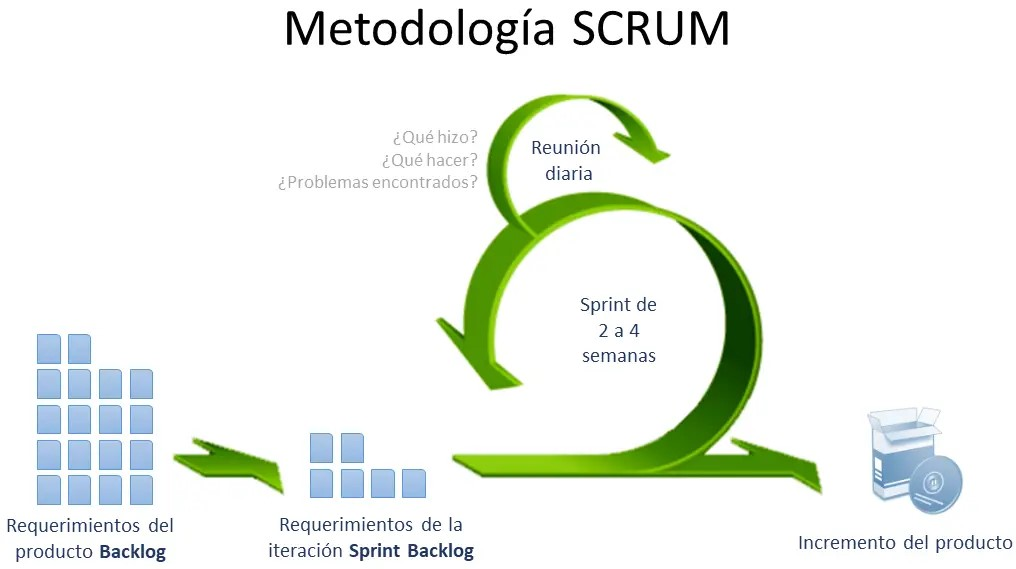
\includegraphics[scale=0.3]{Graphics/SCRUM}
%\caption{Metodología SCRUM [\cite{94}].}
%\label{fig:SCRUM}
%\end{figure}
%
%La Figura \ref{fig:SCRUM} muestra los fundamentos de Scrum. 

Este tipo de metodología trata de realizar entregas del producto final, fijadas en un acuerdo entre el equipo de desarrollo y el \textit{product owner}, para conseguir un resultado completo con cada iteración. Normalmente las iteraciones son de 2 semanas, aunque puede haber equipos que prefieren 3 o 4 semanas.

El \textit{backlog} es un almacén en el cual se encuentran las tareas a realizar, ordenadas por prioridad [\cite{93}]. El equipo de desarrollo es el encargado de añadir y realizar las estimaciones de las tareas, siendo el \textit{product owner} el responsable de priorizar estas. Una vez las tareas se encuentran priorizadas de mayor a menor importancia, según la capacidad del equipo de desarrollo, estos proceden a crear el \textit{sprint}. El \textit{sprint} es el período de tiempo determinado para realizar el trabajo acordado para alcanzar los objetivos propuestos. Es muy importante tener bien definida la tarea, junto con las pruebas de aceptación y una estimación en horas o puntos.

Antes de comenzar un \textit{sprint}, se realiza la reunión llamada \textit{sprint planning}, para seleccionar y comunicar qué tareas es capaz de realizar el equipo, las cuales son seleccionadas del inicio del \textit{backlog}. Una vez finalizado el \textit{sprint} el \textit{product owner} realiza una revisión del trabajo entregado por el equipo de desarrollo y una reunión de retrospectiva en la cual todos los integrantes dejan sus impresiones con el objetivo de mejorar como equipo.

%\item A partir de un identificador, conocer los títulos que posee la persona asociada al identificador.
%\item Autenticar usuarios.
%\item Dado una institución y un rango de fecha listar los diplomas emitidos cumpliendo con la parametrización establecida.
%\item Dado una institución, tipo de diploma, disciplina (carrera / facultad) y un rango de fecha listar los diplomas emitidos cumpliendo con la parametrización establecida.
%\item Dado una institución, disciplina (carrera / facultad) y un rango de fecha listar los diplomas revocados y sus motivos.
%\item Añadir diploma al sistema.
%\item Revocar diploma, pues un título en determinadas situaciones puede ser revocado.

%Tras revisar el abanico de posibilidades metodológicas, y dadas las características del proyecto y del equipo de desarrollo, se ha decidido adaptar el modelo Iterativo a las necesidades del proyecto. Se utilizaron también algunos aspectos del desarrollo ágil, específicamente de la metodología SCRUM, como trabajar en iteraciones y tener alguna parte del sistema funcionando después de cada iteración, para que esto pudiera ser presentado y discutido con el cliente. Esto también ayudó a lograr un proceso de desarrollo más fluido y educativo.

%a las necesidades del proyecto. Siendo el equipo solamente una persona (el autor de 
%este trabajo), no existe ningún rol, pero se mantiene la creación y el mantenimiento del 
%backlog, siguiendo una organización de sprints, permitiendo generar gráficas y ver el 
%estado de trabajo. Si el equipo aumentara en un futuro, se comenzaría a hacer uso de
%los roles definidos en la metodología

%En este proyecto se utilizó un proceso de desarrollo iterativo. Se utilizaron algunos aspectos del desarrollo ágil, como trabajar en iteraciones y tener alguna parte del sistema funcionando después de cada iteración, para que esto pudiera ser presentado y discutido con el cliente. Esto también ayudó a lograr un proceso de desarrollo más fluido y educativo.

%La mayor parte del trabajo del proyecto se realizó en línea. Esto se debió a varias razones, por ejemplo, el hecho de que todos usaban principalmente computadoras de escritorio para el trabajo y se habían acostumbrado a trabajar desde casa durante el covid 19, y las oficinas del cliente estaban a más de una hora de viaje. Los repositorios Git proporcionados por el cliente y la aplicación Telegram sirvieron como plataforma para la cooperación.

\section{Análisis del sistema}
Teniendo en cuenta la propuesta planteada en el capítulo anterior y la metodología de desarrollo adoptada, a continuación se desarrollará el análisis de los principales elementos del sistema. 
%%\subsection{Requerimientos del sistema}
%El Glosario Estándar IEEE de Terminología de Ingeniería de Software define un requisito como condición o capacidad que necesita un usuario para resolver un problema o lograr un objetivo [\cite{95}]. Los requisitos se pueden clasificar en: funcionales y no funcionales.
%
%\subsection{Requisitos funcionales}
%Los requisitos funcionales son capacidades o condiciones que el sistema debe cumplir [\cite{91}]. Su meta principal es identificar y documentar las acciones que en realidad debe ejecutar el sistema para que cumpla con los objetivos planteados al inicio del presente trabajo de diploma.
%
%De acuerdo con los objetivos propuestos el sistema debe ser capaz de:
%
%\begin{enumerate}
%\item A partir de un identificador, conocer los títulos que posee la persona asociada al identificador.
%\item Autenticar usuarios.
%\item Dado una institución y un rango de fecha listar los diplomas emitidos cumpliendo con la parametrización establecida.
%\item Dado una institución, tipo de diploma, disciplina (carrera / facultad) y un rango de fecha listar los diplomas emitidos cumpliendo con la parametrización establecida.
%\item Dado una institución, disciplina (carrera / facultad) y un rango de fecha listar los diplomas revocados y sus motivos.
%\item Añadir diploma al sistema.
%\item Revocar diploma, pues un título en determinadas situaciones puede ser revocado.
%\end{enumerate}
%
%\subsection{Requisitos no funcionales}
%
%Los requisitos no funcionales son propiedades o cualidades que el producto debe tener [\cite{91}]. Debe pensarse en estas propiedades como las características que hacen al producto atractivo, usable, rápido o confiable.
%
%\begin{enumerate}
%\item Requisitos de interfaz y usabilidad:
%	\begin{itemize}
%	\item Tener una interfaz intuitiva y fácil de usar sin necesidad de explicaciones detalladas.
%	\item Contar con una barra de navegación superior y lateral, siguiendo el patrón de los diseños comunes en las aplicaciones actuales.
%	\item Adaptar el contenido adecuadamente al tamaño de pantalla pertinente, ya sea ordenador o dispositivo móvil.
%	\item Usar una paleta de colores consistente.
%	\item Utilizar botones que expresen su función, ya sea a través del ícono o el texto que lo identifica.
%	\item Asegurar que el usuario final sepa dónde se encuentra dentro del flujo procedural de la aplicación, manteniendo una retroalimentación eficiente y completa con dicho usuario.
%	\end{itemize}
%\item Requisitos operacionales:
%	\begin{itemize}
%	\item Ser una aplicación multiplataforma, funcional tanto en sistemas operativos distintos como en dispositivos de diferentes tamaños.
%	\end{itemize}
%\item Requisitos de seguridad:
%	\begin{itemize}
%	\item Tener en cuenta la información visible de los distintos usuarios.
%	\end{itemize}
%\item Requisitos de mantenibilidad y portabilidad:
%	\begin{itemize}
%	\item Tener en cuenta el uso de tecnologías persistentes y una visión de futuro para implementar actualizaciones sin problema alguno.
%	\end{itemize}
%\item Requisitos de recursos:
%	\begin{itemize}
%	\item Ser una aplicación ligera en cuanto al tamaño necesario de almacenamiento.
%	\end{itemize}
%\item Requisitos de rendimiento:
%	\begin{itemize}
%	\item La herramienta debe ser rápida y el tiempo de respuesta debe ser el mínimo posible, al igual que la velocidad de procesamiento de la información.
%	\end{itemize}
%\item Requisitos de disponibilidad:
%	\begin{itemize}
%	\item La aplicación no debe dejar de funcionar aunque se provoquen fallos.
%	\end{itemize}
%\end{enumerate}

%Requisitos no funcionales de Apariencia o Interfaz Externa.
%El usuario debe tener acceso por varias vías a una determinada funcionalidad.
%El sistema debe contener una interfaz sencilla e intuitiva y sea agradable al usuario.
%La herramienta debe utilizar como idioma principal el español, excepto aquellas palabras técnicas 
%que no puedan ser traducidas.
%Utilizar botones que expresen su función, ya sea a través del ícono o el texto que lo identifica.
%Los colores de la interfaz serán agradables, sin mucho brillo que pueda afectar la vista del usuario 
%que tiene sus ojos concentrados en la lectura. 
%Requisitos de Rendimiento.
%La herramienta debe ser rápida y el tiempo de respuesta debe ser el mínimo posible, al igual que la 
%velocidad de procesamiento de la información.

%Fiabilidad en la aplicación: El usuario debe recibir la información mínima sobre
%errores.
%• Seguridad y protección de datos: La aplicación debe cumplir con la normativa
%vigente.
%• Facilidad de uso: El usuario debe ser capaz de usar la aplicación de forma
%intuitiva.
%• Tiempos de respuesta bajos: El usuario no debe recibir esperas prolongadas.
%• Alto nivel de carga: Capacidad para soportar muchos usuarios en la aplicación al
%mismo tiempo.
%• Disponibilidad: La aplicación no debe dejar de funcionar aunque se provoquen
%fallos.
%• Transparencia de acceso: El usuario no debe saber con cuantas entidades se está
%comunicando el sistema.
%• Portabilidad: La aplicación se debe poder usar en cualquier sistema de escritorio.

\subsection{Actores del sistema}
Los actores representan entidades que interactúan con el sistema, un actor del sistema es aquel que se beneficia de los resultados de las funcionalidades del mismo [\cite{91}]. 

Se definen dos tipos de usuarios principales que pueden interactuar con la plataforma: \textbf{anónimos} y \textbf{gestores}. El usuario \textbf{anónimo} es un \textbf{usuario público} que puede acceder sin registrarse a las funcionalidades públicas del sistema.

Los \textbf{gestores} serán usuarios registrados en un sistema de terceros. Estos usuarios tendrán acceso a una sección de \textit{back office} que le permitirá realizar tareas de gestión en la plataforma. Además, contarán con un rol definido en dicho sistema de terceros cuyo rol viajará en la respuesta de autenticación del mismo al nodo cliente (borde del \textit{backend} de la solución a implementar).

\subsection{Casos de uso del sistema}
La forma en que los actores utilizan el sistema puede ser representada a través de los casos de usos [\cite{91}]. Estos últimos son artefactos narrativos que describen, bajo la forma de acciones y reacciones, el comportamiento del sistema desde el punto de vista del actor.

%Los casos de usos identificados en el presente trabajo son enunciados a continuación:
\begin{figure}[!h]
\centering
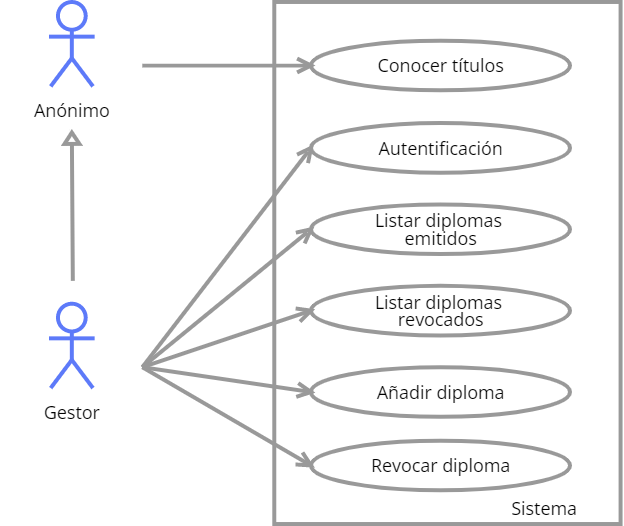
\includegraphics[width=\textwidth]{Graphics/useCasest}
\caption{Diagrama de casos de uso del sistema}
\label{fig:useCases}
\end{figure}

%\subsubsection{Diagrama de casos de uso del sistema}
En la Figura \ref{fig:useCases} se observa el diagrama de casos de uso del sistema a desarrollar. Los diagramas de casos de usos [\cite{91}] son un tipo de diagrama dónde se puede representar el comportamiento esperado del sistema, desde la visión de los usuarios, sin llegar a un alto nivel de especificación acerca de cómo se implementan las acciones. 

%El diagrama de casos de uso del sistema a desarrollar se puede encontrar en la Figura \ref{fig:useCases}.

Los principales elementos que nos encontramos en este tipo de diagramas son:
\begin{itemize}
\item Sistema: Representa con un rectángulo los limites del sistema, los actores se ubican fuera de la figura.
\item Caso de uso: Representado con un óvalo y un texto identificativo, identifican una determinada acción.
\item Actor: Son las entidades externas al sistema que interactúan con el.
\end{itemize}

%\subsubsection{Descripción de los casos de uso del sistema}
A continuación se exponen algunos de los casos de uso de alto nivel, para lograr entender los procesos globales de la aplicación. El resto puede ser encontrado en los anexos \ref{appendix:useCase}.

\begin{table}[!h]
	\begin{center}
		\begin{tabular}{|c|p{10cm}|}
		\hline \textbf{CU1} & Conocer títulos \\ 
		\hline \textbf{Actor} & Anónimo \\ 
		\hline \textbf{Descripción} & El usuario podrá conocer los títulos asociados a una persona al introducir el identificador que representa a la persona.  \\ 
		\hline 
		\end{tabular}
		\caption{Caso de uso: Conocer títulos}
		\label{tab:CU1}
	\end{center}
\end{table}

\begin{table}[!h]
	\begin{center}
		\begin{tabular}{|c|p{10cm}|}
		\hline \textbf{CU2} & Autentificación \\ 
		\hline \textbf{Actor} & Gestor\\ 
		\hline \textbf{Descripción} & El usuario de tipo gestor deberá insertar el nombre de usuario y su contraseña para poder acceder al sistema.\\ 
		\hline 
		\end{tabular}
		\caption{Caso de uso: Autentificación}
		\label{tab:CU2}
	\end{center}
\end{table}

\subsection{Lógica del negocio}
El sistema que se presenta no registrará binarios (copia digital de título, entre otras), sino que los certificados serán representados por propiedades:
\begin{itemize}
\item \textbf{ID}: El identificador de los certificados es con fines de facilitar su búsqueda. No tiene una representación real en un certificado a papel. El campo es generado utilizando la fecha y hora de creación de la credencial. Su estructura es: YYYYMMDDHHMMSS (año, mes, día, hora, minuto y segundo concatenados)
\item \textbf{Certificación}: Título que se le otorga al acreditado.
\item \textbf{Título de oro}: Campo que representa si se alcanzó la distinción.
\item \textbf{Emisor}: Centro que emite el certificado. Ej: Universidad de la Habana.
\item \textbf{Acreditado}: Persona a la que se emite el título.
\item \textbf{Fecha}: Fecha de emisión del documento.
\item \textbf{Creador}: Usuario que creó dicho certificado en la base de datos.
\item \textbf{Secretario, Decano y Rector}: Tres propiedades que guardan los nombres de los funcionarios que validan la Credencial.
\item \textbf{Tomo y folio de facultad y universidad}: Dos propiedades que almacenan Tomo y folio bajo el cual fueron inscritos los documentos tanto en la facultad como en la universidad
\item \textbf{Estado}: Refleja el estado actual del documento.
\item \textbf{Razón de Invalidación}: Refleja, de estar el certificado en estado invalidado, la razón de la decisión.
\end{itemize}

En la aplicación, existirán varios roles con distintas funcionalidades. El personal de las instituciones universitarias podrán realizar consultas más especializadas y gestionar los certificados digitales según el rol que posea, para ello necesitarán iniciar sesión con sus credenciales asignadas. Los roles que se manejarán para los usuarios gestores son los siguientes:

\begin{itemize}
\item \textbf{Administrador de Sistemas}: Encargado de manejar los usuarios que participan en el sistema: crearlos, editarlos, eliminarlos o invalidarle sus credenciales.
\item \textbf{Administrador de Certificados}: Usuario que tiene los permisos para gestionar los certificados: crearlos, editarlos, eliminarlos o invalidarlos. Este rol no valida los certificados.
\item \textbf{Secretario General}: Usuario que tiene los permisos para validar certificados recién creados. Puede invalidar los certificados que encuentre inconsistentes.
\item \textbf{Decano de Facultad}: Usuario que tiene los permisos para validar certificados aprobados por el Secretario General. Puede invalidar los certificados que encuentre inconsistentes.
\item \textbf{Rector de Universidad}: Usuario que tiene los permisos para validar certificados aprobados por el decano. Es el último eslabón para hacer un certificado válido. Puede invalidar los certificados que encuentre inconsistentes.
\item \textbf{Inválido}: Usuario al que le fueron retirados sus privilegios por un administrador de sistema.
\end{itemize}

Los certificados pueden tener cinco estados:
\begin{itemize}
\item \textbf{Inválido}: El certificado fue invalidado por un usuario gestor con los permisos adecuados.
\item \textbf{Creado}: El documento fue creado, pero no posee ninguna firma de validación.
\item \textbf{Firmado por Secretario}: El documento fue validado por un usuario gestor con rol de `secretario'.
\item \textbf{Firmado por Secretario y Decano}: El documento fue validado por un usuarios gestores con rol `secretario' y `decano'.
\item \textbf{Válido}: El certificado fue validado por usuarios gestores con rol `secretario', `decano' y `rector'.
\end{itemize}
%Para la emisión de los certificados, primeramente el administrador de certificados debe insertar el título. Una vez insertado, el decano debe aprobar o validar este certificado, el cual deberá entonces ser validado por el secretario general para finalmente ser validado por el rector. Para la validez del título debe haber sido validado por las tres últimas entidades mencionadas y siguiendo el orden en el que fueron nombradas.

\subsection{Historias de usuario}
Las historias de usuario se usan, en el contexto de la ingeniería de requisitos ágil, como una herramienta de comunicación que combina las fortalezas de ambos medios: escrito y verbal. Describen, en una o dos frases, una funcionalidad de \textit{software} desde el punto de vista del usuario, con el lenguaje que éste emplearía. Se enfocan en qué necesidades o problemas soluciona lo que se va a construir.

A continuación se exponen algunos de las historias de uso de alto nivel, las demás pueden ser encontradas en los anexos \ref{appendix:useHistory}.

\begin{table}[!h]
	\begin{center}
		\begin{tabular}{|c|p{10cm}|}
		\hline \textbf{H.U-1} & Conocer títulos \\ 
		\hline \textbf{Usuario} & Anónimo\\ 
		\hline \textbf{Descripción} & Como usuario anónimo quiero poder conocer los certificados de una persona para poder observar las habilidades y estudios de esa persona. \\ 
		\hline 
		\end{tabular}
		\caption{Historia de Usuario: Conocer títulos}
		\label{tab:HU1}
	\end{center}
\end{table}

\begin{table}[!h]
	\begin{center}
		\begin{tabular}{|c|p{10cm}|}
		\hline \textbf{H.U-2} & Autentificación \\ 
		\hline \textbf{Usuario} & Gestor \\ 
		\hline \textbf{Descripción} & Como usuario gestor quiero poder autenticarme para poder tener acceso al sistema. \\ 
		\hline 
		\end{tabular}
		\caption{Historia de Usuario: Autentificación}
		\label{tab:HU2}
	\end{center}
\end{table}

\begin{table}[!h]
	\begin{center}
		\begin{tabular}{|c|p{10cm}|}
		\hline \textbf{H.U-3} & Cerrar sesión \\ 
		\hline \textbf{Usuario} & Gestor \\ 
		\hline \textbf{Descripción} & Como usuario gestor quiero poder cerrar la sesión actual para poder salir de forma segura del sistema. \\ 
		\hline 
		\end{tabular}
		\caption{Historia de Usuario: Cerrar sesión}
		\label{tab:HU3}
	\end{center}
\end{table}

\subsection{Planificación de desarrollo}
Siendo el equipo solamente una persona (el autor de este trabajo), no existe ningún rol, pero de acuerdo con Scrum, se mantiene la creación y el mantenimiento del \textit{backlog}, siguiendo una organización de \textit{sprints}, permitiendo tener alguna parte del sistema funcionando después de cada iteración, para que esto pudiera ser presentado y discutido con el cliente \footnote{El Instituto de Criptografía de la Universidad de La Habana toma el rol del cliente.}. Si el equipo aumentara en un futuro, se comenzaría a hacer uso de los roles formalmente definidos en la metodología.

La fecha final del proyecto será acorde a la fecha límite de entrega de la convocatoria ordinaria del Trabajo de Fin de Grado. Por tanto, se ha establecido la duración de los sprints en 2 semanas, teniendo cada uno una carga de 34h aproximadamente por \textit{sprint}. En la tabla \ref{tab:sprints} puede verse una planificación inicial. Esta planificación es susceptible a cambios, así como la fecha de finalización podría ser cambiada.

%        Para la administración de tareas, se ha utilizado la herramienta Jira, creada por la 
%empresa Atlassian, que permite realizar una gestión ágil del proyecto. Jira crea 
%Aplicación web para la gestión de clubes de fútbol
%48
%automáticamente el backlog, que es la lista de trabajo donde se encuentran las tareas 
%encontrándose arriba las más importantes por el propietario del producto [40].
%Dentro de Jira, se puede crear distintos sprints, explicado anteriormente en el punto 
%3.4.1, indicando las fechas y las tareas que existen. Además, permite visualizar los 
%informes del sprint, siendo muy útiles para el equipo de desarrollo y sobre todo para el 
%Scrum máster.
%La plataforma no solo permite la creación y el seguimiento de los sprints, también es 
%posible realizar un seguimiento de los bugs registrados.

\begin{table}[!h]
	\begin{center}
		\begin{tabular}{|p{2cm}|p{3cm}|p{3cm}|p{3.8cm}|}
		\hline \textbf{Sprint} & \textbf{Comienzo} & \textbf{Final} & \textbf{H.U a desarrollar} \\ 
		\hline Sprint 0 & 1/09/2022  & 15/09/2022 & -\\ 
		\hline Sprint 1 & 15/09/2022 & 29/09/2022 & H.U-1\\ 
		\hline Sprint 2 & 29/09/2022 & 13/10/2022 & H.U-2, H.U-3\\ 
		\hline Sprint 3 & 13/10/2022 & 27/10/2022 & H.U-4\\ 
		\hline Sprint 4 & 27/10/2022 & 10/11/2022 & H.U-5, H.U-6, H.U-7\\ 
		\hline Sprint 5 & 10/09/2022 & 24/10/2022 & H.U-8\\ 
		\hline 
		\end{tabular}
		\caption{\textit{Backlog} inicial}
		\label{tab:sprints}
	\end{center}
\end{table}

Debido a la poca experiencia del autor con las tecnologías establecidas por el cliente, se realizará un \textit{sprint} 0 con el objetivo de analizar y aprender estas tecnologías para la correcta realización del proyecto.

\section{Diseño del sistema}
Tras el apartado de análisis, en el que se ha establecido cuales son los elementos que se desean incluir en el sistema, se desarrolla a continuación el apartado, en el que se explica cómo se quieren llevar a cabo los requisitos.

\subsection{Arquitectura del sistema}
La arquitectura de un \textit{software} se encarga de entender cómo debe organizarse el sistema y cómo tiene que diseñarse la estructura global del mismo [\cite{91}]. Constituye el enlace crucial entre el diseño y la ingeniería de requisitos, ya que identifica los principales componentes estructurales en un sistema y la relación entre ellos. La salida del proceso de diseño arquitectónico consiste en un modelo arquitectónico que describe la  forma en que se organiza el sistema como un conjunto de componentes en comunicación. La arquitectura de \textit{software} representa un elemento fundamental pues afecta el desempeño del sistema, así como su capacidad de distribución y mantenimiento.

Según [\cite{99}], la arquitectura de un sistema puede basarse en un patrón o un estilo arquitectónico particular. Un patrón arquitectónico es una descripción de una organización del sistema, captan la esencia de una arquitectura usada en diferentes sistemas de \textit{software}.

\begin{figure}[htbp]
\centering
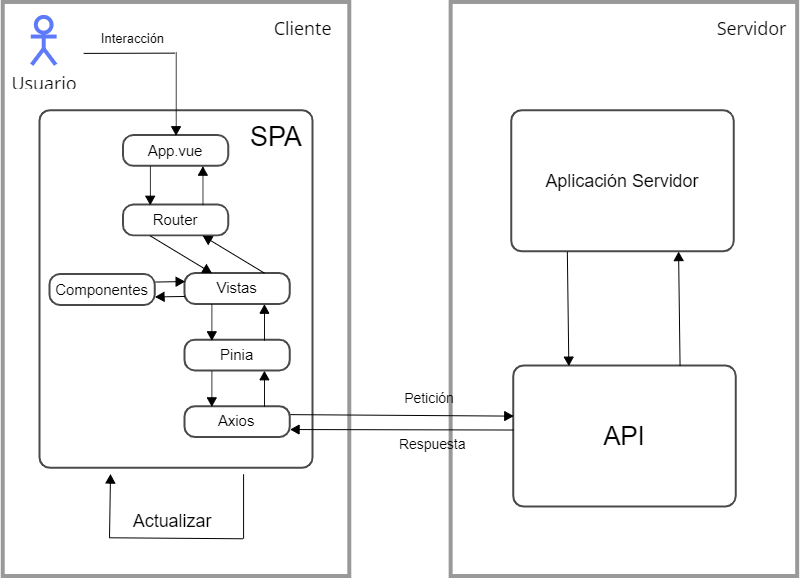
\includegraphics[width=\textwidth]{Graphics/mySPAtt}
\caption{Arquitectura de la solución}
\label{fig:spa}
\end{figure}
%Para empezar la sección de diseño, se va a exponer la arquitectura del sistema que se va a
%implementar, destacando dos aspectos relevantes, el patrón de diseño Modelo Vista VistaModelo (MVVM) y la denominada arquitectura backendless

%Para la realización del sistema se apuesta por la división de 3 niveles: presentación, lógica de negocio y persistencia. 
%
%\begin{figure}[htp]
%\centering
%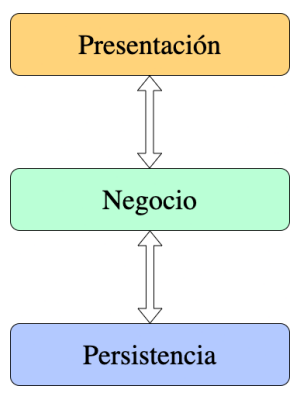
\includegraphics[scale=0.9]{Graphics/levels}
%\caption{Arquitectura del sistema}
%\label{fig:3levels}
%\end{figure}
%
%La arquitectura de tres niveles organiza el sistema en distintos niveles lógicos y físicos. El nivel de presentación, donde se encuentra la interfaz del usuario, en la cual se enfoca el presente trabajo; el nivel de negocio, donde se encuentra toda la lógica para procesar los datos y, por último, el nivel de persistencia, donde se almacenan los datos [\cite{96}]. Cada nivel puede encontrarse en una infraestructura distinta y desacoplado de los demás, por lo que estos niveles pueden escalar y actualizarse según sea necesario. Suele haber una confusión entre nivel y capa. La división en capas es simplemente la división funcional, sin embargo, la división en niveles es una división funcional y de infraestructura. Esto quiere decir que el \textit{software} se ejecuta en distintas máquinas y no en la misma.
%
%El nivel de presentación es la encargada de mostrar al usuario la información, interactuar con él y ajustar estos datos a las especificaciones que son demandadas por la capa de negocio. En el caso de nuestra aplicación este nivel se ejecuta en el navegador web. 
%
%El nivel de negocio es el encargado de facilitar al nivel de presentación los datos necesarios, a la vez que recolecta los datos aportados por este para procesarlos. Este nivel está también conectado con el nivel de persistencia, enviándole peticiones para almacenar o recuperar datos de este [\cite{96}].
%
%El nivel de persistencia es donde residen los datos y generalmente está formada por un gestor encargado de realizar el almacenamiento de datos. Este nivel recibe las peticiones de negocio, quien le dice qué datos necesita o qué datos tiene que almacenar. El nivel de persistencia no se puede comunicar directamente con el nivel de presentación, siempre debe de comunicarse con negocio previamente [\cite{96}]. 
%
%%Vue.js utiliza una arquitectura basada en componentes, separando así grandes trozos de código en componentes más pequeños. Además, en Vue.js, todo es un componente, y cada componente está escrito con HTML, CSS y JavaScript, lo que favorece la legibilidad y la simplicidad.
%%
%%El back-end proporcionará endpoints para el registro y el acceso de un usuario, así
%%como una API CRUD para el manejo de notas (crear, recuperar, actualizar y eliminar);
%%y será el front-end el que haga uso de estos puntos de acceso para darle al usuario un
%%servicio de notas online.
%
%Como mencionamos previamente, el presente trabajo de diploma se enfoca en el desarrollo del nivel de presentación. 

El empleo de Vue para el desarrollo de la aplicación permite dividir la aplicación en distintos bloques funcionales independientes llamados componentes, esto se suele denominar arquitectura de componentes[\cite{50}]. Todos los componentes relacionados entre sí se agrupan y se comunican entre sí para realizar las tareas. Esta arquitectura permite generar aplicaciones a base de la reutilización de estos componentes, evitando tener código redundante.

La arquitectura de la solución propuesta es una arquitectura \textit{N-Layer} adaptada a las características del proyecto (ver Figura \ref{fig:spa}). Cuando el usuario accede en el navegador a la aplicación, internamente al componente raíz App.vue se le transfiere un componente enrutador, el cual debe hacer uso de las rutas definidas para cargar la vista deseada por el usuario. Las vistas son las diferentes páginas del sitio Web \footnote{Página principal, la lista de usuarios, la lista de certificados, entre otras} que se encargan de gestionar los datos a los distintos componentes que la conforman. Los componentes son pequeños bloques funcionales de código que son comunes en las diferentes vistas (como por ejemplo la barra de navegación, los botones, entre otras.); su utilidad está dada por el hecho de que son definidos una sola vez y luedo son reutilizados en distintas ocasiones. Para trabajar con datos, las vistas invocan a las funciones de Pinia, las cuales se encargan de realizar las peticiones a la API, la cual escucha y responde a las solicitudes de los clientes. La capa encargada de manejar las solicitudes a la API fue denominada Custom, esta capa es la encargada de realizar las acciones necesarias para recopilar los datos y enviar la respuesta de vuelta a Pinia. Cuando Pinia ya ha obtenido la respuesta, este envía los datos a la vista, quien muestra al usuario el contenido de la ruta a la que accedió.

%La arquitectura de este nivel está basada en componentes. Todos los componentes relacionados entre sí se agrupan y se comunican entre sí para realizar las tareas. Por ejemplo, el componente de carga interactúa con el componente de inicio cuando se realiza la carga para actualizar la interfaz de usuario. Toda la funcionalidad se realiza en estructuras de componentes pequeños y estos componentes están diseñados para ser reutilizables.

%La arquitectura de la interfaz de usuario propuesta también se basa en las arquitecturas cliente-servidor. Las SPA se caracterizan por cargar todos los recursos de la aplicación Web en la consulta inicial, como si se tratara sólo de una página. Los componentes cambian dinámicamente a medida que el usuario va interaccionando con ellos. Esto proporciona una interfaz de usuario más rápida y fluida, ya que todas las representaciones se realizan localmente en el navegador del usuario. La página solicita nueva información del servidor cuando los datos almacenados en la página ya no se corresponden con los que se encuentran en el servidor. (Ver Figura \ref{fig:spa}).

\subsection{Patrones de diseño}

La arquitectura es necesaria para comprender el sistema, organizar el desarrollo, fomentar la reutilización y hacer evolucionar el sistema. Para definirla es muy importante tener en cuenta un patrón de diseño o modelo de abstracción que nos sirva para poder estructurar de manera eficaz todos los componentes de la aplicación, tanto la parte de la interfaz (vista), como la de la lógica (controlador) y la del modelo de datos (modelo).

%necesario seleccionar y combinar patrones. Los patrones de diseño constituyen la base para la búsqueda de soluciones a problemas comunes en el desarrollo de software y otros ámbitos referentes al diseño de interacción o interfaces. Un patrón de diseño es una solución a un problema de diseño; facilitan la reusabilidad, extensibilidad y mantenimiento. 

\subsubsection{Patrón MVVM}

El patrón Modelo Vista Vista Modelo o en inglés Model View ViewModel (MVVM) se diferencia del clásico Modelo Vista Controlador (MVC) [\cite{45}]. En el MVC, es el controlador (el componente encargado de toda la lógica de la aplicación que enlaza la vista con el modelo) quien debe actualizar manualmente los cambios producidos en el modelo o en la vista de manera independiente, mientras que en el patrón MVVM, estos cambios se actualizan automáticamente gracias al componente VistaModelo. Es decir, si se produce un cambio en la vista, los datos son actualizados de forma automática en la parte del modelo, y viceversa.

Por ejemplo, el entorno de desarrollo Vue está centrado en el componente Vista-Modelo del patrón MVVM [\cite{49,47}], que se encarga del trabajo realizado por el controlador en el diseño MVC, pero enlazando los datos entre la vista y el modelo de forma reactiva, simple y flexible.

\begin{figure}[htbp]
\centering
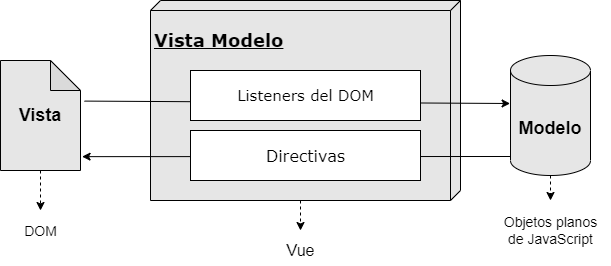
\includegraphics[width=\textwidth]{Graphics/mvvm}
\caption{Patrón de diseño MVVM en Vue [\cite{47}].}
\label{fig:vmmv}
\end{figure}


%Todos estos son marcos que utilizan un patrón de diseño Model-View-Viewmodel (MVVM). Aquí, el modelo representa la lógica comercial de back-end, la vista representa el diseño de la interfaz de usuario y el modelo de vista representa el código intermediario entre los dos, que maneja la lógica de la vista. Ver figura 4.
%
El objetivo principal de una implementación de MVVM es separar la lógica de la interfaz de usuario de la lógica empresarial. Esto nos trae varias ventajas, una de ellas es la separación de preocupaciones. Esto significa que evita el código estrechamente acoplado y resistente al cambio, el cual a menudo puede causar problemas durante el mantenimiento o la actualización. Otra ventaja importante es que permite a un solo desarrollador poder desarrollar y probar una aplicación completa sin tener mucha experiencia con el diseño de UI como es el caso del autor de este proyecto.
%
%Una de las características clave de MVVM Frameworks es el enlace de datos entre los datos de la vista y la lógica del modelo de vista. El enlace de datos es la práctica de vincular un proveedor de datos y un consumidor de datos, y con esto permitir una conexión bidireccional. Esto es muy útil en el contexto del desarrollo de Frontend porque desea vincular la interfaz de usuario a la lógica, pero estos generalmente están en dos idiomas diferentes, por ejemplo, HTML y JavaScript. Al usar el enlace de datos, los elementos de la interfaz de usuario en la vista se pueden cambiar dinámicamente desde la lógica en el modelo de vista.
%
%El patron Modelo Vista Vista Modelo o en inglés Model View ViewModel, es una variación del MVC que está diseñado para plataformas de desarrollo de interfaz de usuario modernas donde la vista es responsabilidad de un diseñador en lugar de un desarrollador. MVVM se basa en un mecanismo general de enlace de datos que facilita el desarrollo de la capa de separación de vista desde el resto del patrón mediante la eliminación de todo el código subyacente de la capa de la vista. 
%
%El modelo, encapsula la lógica de negocio y datos. La lógica empresarial se define como cualquier lógica de aplicación que se ocupa de la recuperación y gestión de datos de la aplicación y de asegurar que las reglas del negocio que garanticen la coherencia de los datos y la validez se cumplan. Para maximizar las oportunidades de reutilización, los modelos no deben contener ningún caso de uso o conducta específica del usuario o lógica de la aplicación. 
%
%La vista, encapsula la interfaz de usuario y la lógica de la interfaz de usuario. Las vistas definen la interfaz de usuario específica para una parte de la aplicación, son normalmente los controles que se han diseñado para funcionar bien cuando se une a un ViewModel.
%
%El viewmodel, encapsula la lógica de presentación y estado. Lógica de presentación se define como la lógica de la aplicación que se ocupa de casos de uso de la aplicación (o casos de usuario, tareas de usuario, flujo de trabajo, etc.) y define el comportamiento lógico y la estructura de la aplicación. Para maximizar las oportunidades de reutilización, el ViewModel no debe tener ninguna referencia a las clases específicas de interfaz de usuario, elementos, controles o comportamiento.
%

%El modo MVVM es el mismo que el modo MVC, el propósito principal es separar la vista (Vista) del modelo (Modelo), hay varias ventajas
%
%Acoplamiento bajo: las vistas pueden ser independientes de los cambios y modificaciones del modelo. Un modelo de vista se puede vincular a diferentes vistas. Cuando la vista cambia, el modelo puede permanecer sin cambios, y cuando el modelo cambia, la vista también puede permanecer sin cambios.
%Reutilizable: puede poner algo de lógica de vista en un modelo de vista y permitir que muchas vistas reutilicen esta lógica de vista.
%Desarrollo independiente: los desarrolladores pueden centrarse en la lógica empresarial y el desarrollo de datos (ViewModel), y los diseñadores pueden centrarse en el diseño de páginas.
%Comprobable: la interfaz siempre ha sido difícil de probar, pero ahora la prueba se puede escribir para ViewModel.

%Modelo: capa de modelo, que representa objetos JavaScript aquí
%Vista: capa de vista, donde DOM (elemento de manipulación HTML) se representa aquí
%ViewModel: middleware que conecta vistas y datos, Vue.js es el implementador de la capa ViewModel en MVVM
%En la arquitectura MVVM, los datos y la vista no pueden comunicarse directamente y solo pueden comunicarse a través de ViewModel, y ViewModel define un observador
%
%ViewModel puede observar cambios de datos y actualizar el contenido correspondiente a la vista
%ViewModel puede monitorear cambios en la vista y notificar cambios en los datos
%En este punto, entendemos que Vue.js es un implementador de MVVM, y su núcleo es implementar el monitoreo DOM y el enlace de datos.

%Entre los elementos de un patrón se encuentran: Nombre (describe el problema de 
%diseño), Problema (describe cuándo aplicar el patrón) y Solución (describe los elementos que 
%componen el diseño, sus relaciones, responsabilidades y colaboración).
%
%En aplicaciones grandes, es posible que necesitemos dividir la aplicación en partes más pequeñas y solo cargar un componente del servidor cuando sea necesario. Para hacerlo más fácil, Vue le permite definir su componente como una función de fábrica que resuelve de forma asíncrona la definición de su componente. Vue solo activará la función de fábrica cuando el componente deba renderizarse y almacenará en caché el resultado para futuros renderizados.

%Los componentes y contenedores no son más que el patrón de diseño Mediator. Donde los componentes serán los que se encargar de pintar, podrán tener lógica de pintado, pero muy poca. Reciben datos y los pintas, nada más. Los contenedores son aquellos que orquestan a los componentes y les pasan los datos. Suelen tener más lógica pero no suelen tener ni estilos visuales ni markup.
%
%Los componentes se comunican con los contenedores mediante eventos, y los contenedores se comunican con los componentes mediante props. Esto hace que los tests sean mucho más fáciles, los componentes estén más desacoplados y si falla algo en cuanto a la orquestación, sabremos que tenemos que mirar el contenedor.
%

%Encapsulación: propone esconder algunos componentes, permitiendo sólo accesos estilizados al 
%objeto. Se hace uso de este patrón en casi todas las clases que componen la solución, permitiendo que 
%estas solo posean como elementos públicos aquellos que son exclusivamente necesarios (24).
%Subclase: propone heredar miembros por defecto de una superclase, seleccionando la implementación 
%correcta a través de resoluciones sobre qué implementación debe ser ejecutada. Se puede encontrar este 
%patrón con más fuerza en las entidades de negocio que por su conceptualización las funciones y la 
%información que almacenan pueden estar diferenciadas en cierta medida (24).
%Fábrica: provee de una interfaz para crear familias de objetos relacionados o dependientes sin 
%especificar los tipos concretos de clases. Su uso se encuentra centrado a la creación de los conectores 
%correspondientes al acceso a datos que se esté utilizando, así como en la obtención de los servicios a 
%utilizar (24).

%Vue: permita que el cliente almacene el estado local de una manera funcional basada en patrones de observadores
%Este patrón de diseño le permite suscribirse y emitir eventos desde componentes de su aplicación.
\subsubsection{Patrones GRASP}
Los patrones GRASP (Patrones Generales de Software para Asignación de Responsabilidades) describen los principios fundamentales de diseño de objetos para la asignación de responsabilidades. Las responsabilidades  están relacionadas con las obligaciones de un objeto en cuanto a su comportamiento [\cite{97}]. Entre los patrones GRASP empleados en la solución encontramos:

\begin{itemize}
\item Bajo Acoplamiento: El acoplamiento es una medida de la fuerza con que una clase está conectada a otras clases, con que las conoce y recurre a ellas. El bajo acoplamiento soporta un diseño de clases más independientes, que reducen el impacto de cambios, y permite que sean más reutilizables.

La arquitectura de software basada en componentes permite un bajo acoplamiento entre sus componentes. Estos pueden ser creados, modificados o eliminados en cualquier momento, lo que proporciona que la dependencia entre ellos sea baja.

\item Alta Cohesión: La cohesión es una medida de la fuerza con la que se relacionan las clases y el grado de focalización de las responsabilidades de un elemento. Cada elemento del diseño debe realizar una labor única dentro del sistema, no desempeñada por el resto de los elementos, y auto-identificable. Una clase con baja cohesión realiza muchas labores no relacionadas o realiza demasiado trabajo.

La arquitectura de software basada en componentes permite la organización del trabajo en cuanto a la estructura del proyecto y la asignación de responsabilidades con una alta cohesión. Cada componente realiza solo las funcionalidades para las cuales fueron creados, colaborando entre ellos para cumplir con el resto de las funcionalidades, generando un bajo acoplamiento y fomentando la reutilización. Esto hace posible que el sistema sea flexible a cambios sustanciales con efecto mínimo
\end{itemize}

\subsubsection{Patrones GoF}
Los patrones GoF (Patrones de la ``pandilla de los cuatros'') son los más utilizados en la implementación de \textit{software} [\cite{97}]. Los patrones GoF utilizados en la propuesta de solución son los siguientes:

\begin{itemize}
\item Singleton (Instancia Única): Su propósito es asegurar que una clase tenga una única instancia y proporcionar un punto de acceso global a dicha instancia.

En la solución se ve presente al instanciar el hilo principal de la aplicación, la clase encargada de la autenticación de usuarios y la clase encargada de la comunicación, garantizando un único punto de acceso y evitando la replicación de hilos y proceso.

\item Observer (Observador): Este patrón define una dependencia de uno-a-muchos entre objetos, de manera que cuando un objeto cambie de estado se notifique y actualicen automáticamente todos los objetos que dependen de él.

Los servicios de gestión de estado de Vue utilizan el patrón de observador, permitiendo al cliente almacenar el estado local de una manera funcional [\cite{52}]. El patrón se utiliza como soporte para que el sistema pueda comunicarse con una API externa accediendo a los datos brindados por el paquete de servicios (Pinia). En esta solución permite mantener consistencia entre objetos relacionados sin aumentar el acoplamiento entre clases.

\end{itemize}
%A continuación se presenta los patrones de diseño GoF que fueron seleccionados para utilizar como 
%parte de la solución:
%Singleton: Su propósito es asegurar que una clase tenga una única instancia y proporcionar un 
%punto de acceso global a dicha instancia en este caso esa función la realiza la clase “MainController”. 
%De esta forma se logra crear una variable global, que hace el objeto accesible y para que sea posible 
%instanciarla sólo una vez. En consecuencia hay un acceso controlado a dicha única instancia, y se 
%gestionan de manera centralizada los recursos utilizados.
%Follwing the singleton pattern, we created a new file in which we created a new instance
%of Axios that could be reused and imported whenever needed
%
%Decorator: Añade capacidad de desplazamiento a una vista. Para este caso facilita los cambios 
%dinámicos en la apariencia de la aplicación cuando se aplica la configuración de alto contraste para 
%mejorar la lectura de los discapacitados visuales. 
%Observer: Se utiliza para definir una dependencia de uno-a-muchos entre objetos, de forma que 
%cuando un objeto cambie de estado se notifique y actualicen automáticamente todos los objetos que 
%dependen de él. En esta solución permite mantener consistencia entre objetos relacionados sin 
%aumentar el acoplamiento entre clases.

%Observer 
%31
%Este patrón define una dependencia de uno-a-muchos entre objetos, de manera que 
%cuando un objeto cambia de estado, todos sus dependientes son notificados y 
%actualizados automáticamente. En la solución se ve presente cuando ocurre cualquier 
%evento que el usuario necesite conocer, automáticamente la consola es notificada para 
%que actualice su estado, también se puede presenciar en el módulo de creación de salvas 
%periódicas, cuando cambia el estado de la configuración, automáticamente es enviada la 
%notificación para realizar o no la creación de las salvas.
%Singleton
%Es un patrón creacional cuyo principal objetivo es garantizar que una clase solo tenga
%una única instancia, proporcionando un punto de acceso global a la misma. En la solución 
%se ve presente al instanciar el hilo principal de la aplicación, la clase encargada de la 
%autenticación de usuarios y la clase encargada de la comunicación, garantizando un 
%único punto de acceso y evitando la replicación de hilos y proceso

%2.4.1 Patrones GRASP24
%Una de las actividades más complicadas en Orientación de Objetos consiste en elegir las clases 
%adecuadas y decidir como estas clases deben interactuar. 
%Experto: La responsabilidad de realizar una labor es de la clase que tiene o puede tener los datos 
%involucrados (atributos). Una clase, contiene toda la información necesaria para realizar la labor que tiene 
%encomendada.
%Creador: El patrón Creador guía la asignación de responsabilidades relacionadas con la creación de 
%objetos. El propósito fundamental de este patrón es encontrar la clase responsable de crear una nueva 
%instancia de determinada clase.
%Controlador: Un Controlador es un objeto que se encarga de manejar un evento del sistema. Este no 
%realiza mucho trabajo por sí mismo, sino que delega en otros objetos, coordina y controla el trabajo que se 
%necesita hacer.

%2.4.2 Patrones GoF
%25
%Singleton (Instancia Única): Está diseñado para restringir la creación de objetos pertenecientes a una 
%clase a un único objeto. Asegura que una clase tiene una sola instancia y proporciona un punto de acceso
%global a ella.
%Factory Method (Método de Fabricación): Define una interfaz para crear un objeto dejando a las 
%subclases decidir al tipo específico al que pertenecen.
%Algunas de las ventajas de este patrón son:
%Centralización de la creación de objetos.
%Facilita la escalabilidad del sistema.
%El usuario se abstrae de la instancia a crear.
%Facade (Fachada): Simplifica los accesos a un conjunto de clases relacionadas proporcionando una
%única clase que todos utilizan para comunicarse con dicho conjunto de clases.

%Patrones GRASP5
%(Patrones Generales de Software para Asignación de Responsabilidades):
%Según (Grosso 2011), son patrones basados en la asignación de responsabilidades a objetos. Es una 
%buena práctica para el desarrollo eficaz de la Programación Orientada a Objetos (POO).
%• Experto: consiste en asignar la responsabilidad de realizar una labor a la clase que tiene o puede 
%tener los datos involucrados
%
%Creador: consiste en asignar a una determinada clase B la responsabilidad de crear una instancia 
%de la clase A al ocurrir alguna de las siguientes circunstancias
%
%Bajo acoplamiento: consiste en asignar una responsabilidad a una clase de manera que el 
%acoplamiento permanezca bajo. Una clase con bajo (o débil) acoplamiento no depende de muchas 
%otras clases
%
%La arquitectura de software basada en componentes permite un bajo acoplamiento entre sus 
%componentes. Estos pueden ser creados, modificados o eliminados en cualquier momento, lo que 
%proporciona que la dependencia entre ellos sea baja.
%• Alta cohesión: consiste en asignar una responsabilidad de manera que la cohesión permanezca 
%alta. La cohesión es una medida de la fuerza con la que se relacionan las responsabilidades de un 
%elemento.
%La arquitectura de software basada en componentes permite la organización del trabajo en cuanto a la 
%estructura del proyecto y la asignación de responsabilidades con una alta cohesión. Cada componente 
%realiza solo las funcionalidades para las cuales fueron creados, colaborando entre ellos para cumplir con 
%el resto de las funcionalidades, generando un bajo acoplamiento y fomentando la reutilización. Esto hace 
%posible que el sistema sea flexible a cambios sustanciales con efecto mínimo

%Patrones GoF6
%(Patrones de la “pandilla de los cuatros”):
%Los patrones GoF son los más utilizados en la implementación de algún software, se clasifican por su 
%propósito en creacionales, estructurales y de composición, mientras que respecto a su ámbito se clasifican 
%en clases y objetos (Gamma et al. 1997). Los patrones GoF utilizados en la propuesta de solución son los 
%siguientes:
%• Decorator (Decorador): proporciona metadatos adicionales a las clases que determinan cómo el 
%componente se debe procesar, instanciar y usar en tiempo de ejecución.
%
%• Observer (Observador): se utiliza como soporte para que el sistema pueda comunicarse con una 
%API7
%(Interfaz de Programación de Aplicaciones) externa accediendo a los datos brindados por el 
%Paquete de Servicios

%• Singleton (Instancia única): se encarga de asegurar que una clase tenga una sola instancia y 
%que proporcione un punto de acceso global a ella. El uso de este patrón es necesario cuando 
%existen clases que tienen que gestionar de manera centralizada un recurso.
%\subsection{Principios de diseño}
%El diseño de la interfaz orienta al usuario respecto al lugar donde se encuentre, mediante la barra de título. 
%Los mensajes de ayuda, así como el del botón cerrar provee al usuario de una respuesta inmediata; el
%sistema cuenta con un área de mensaje de estado donde se muestra información sobre la tarea que el 
%usuario está realizando en ese momento. 
%La interfaz propuesta posee una barra de herramienta donde aparecen las funcionalidades más usadas 
%por el usuario; cuenta con un panel de control donde estarán ubicados los diferentes parámetros que se 
%corresponden con la ejecución de las funcionalidades y los elementos incluidos en esta barra de 
%herramientas poseen un tamaño razonable para que no resulte difícil dar clic sobre ellos. Los íconos 
%utilizados para la representación de estas funcionalidades no se utilizan para otra cosa que no sea su 
%finalidad prevista y los colores utilizados en los mismos son de gran contraste entre ellos y respecto al 
%color de fondo. Se le da al usuario la posibilidad de cerrar la aplicación en el momento que así lo desee,mostrándole un mensaje de confirmación de la acción en caso que el usuario no esté seguro del 
%procedimiento.
%La interfaz le da la posibilidad al usuario de acceder a la ayuda del sistema en caso que este se encuentre 
%desorientado. La información se sitúa con sutileza para facilitar la interacción del usuario con la aplicación, 
%con un tamaño de letra para los íconos y menús (MS Shell Dlg 2), tratando de variar al mínimo. Para el 
%color de las letras se utiliza el negro que se distingue sobre el fondo gris y esto le aporta seriedad a las 
%aplicaciones de este tipo. El diseño proporciona una serie de menús desplegables que solo se muestran
%cuando el usuario hace clic en uno de ellos; los mismos están visibles en todo momento y son accesibles
%desde el teclado.

%Un principio de diseño es un conjunto de buenas prácticas para la actividad del diseño, 
%de las cuales se pueden desprender la identificación de piezas en las cuales 
%descomponer el sistema, la asignación de responsabilidades a esas piezas, garantizando 
%la manera en que interactúan unas con otras [38].
%A continuación, se mencionan los principios de diseño utilizados en el desarrollo de la 
%aplicación:
%Single responsibility principle (Principio de única responsabilidad)
%Define que una clase o función de una clase deben tener una única razón para cambiar. 
%Se debe analizar si existe más de una posible razón que puedan generar cambios en 
%una clase o una función, si es así, puede ser que esta se esté dedicando a más de un 
%tipo de responsabilidad, con lo cual, será más probable que cambie a menudo y será 
%potencialmente menos reutilizable. Este principio se utiliza en la solución en general, 
%donde las clases tienen responsabilidad única, por ejemplo, la clase Client tiene la única 
%responsabilidad relacionada con la comunicación con el Servidor

%Ley de Demeter 
%Este principio establece que las operaciones de una clase, solamente deberían efectuar 
%llamadas a objetos que cumplan una de las 4 características siguientes: a sí mismos, a 
%objetos pasados como argumento, a objetos creados por ella y a objetos con los cuales 
%tiene relaciones directas.
%Once and Only Once Rule 
%Este principio establece la no repetición de una misma responsabilidad en más de una 
%clase o módulo, en la medida en que alguna función es repetida en un mayor número de 
%lugares, a la hora de modificar esa función, se pueden quedar varias de las piezas 
%afectadas sin actualizar el cambio. Si por el contrario esa regla o función estuviera 
%implementada en un único lugar, efectuar un cambio en ese único lugar, haría que el 
%cambio quedara integrado al sistema consistentemente.

%\subsection{Diagramas de diseño}

\subsection{Elementos de seguridad}
\begin{figure}[!h]
\centering
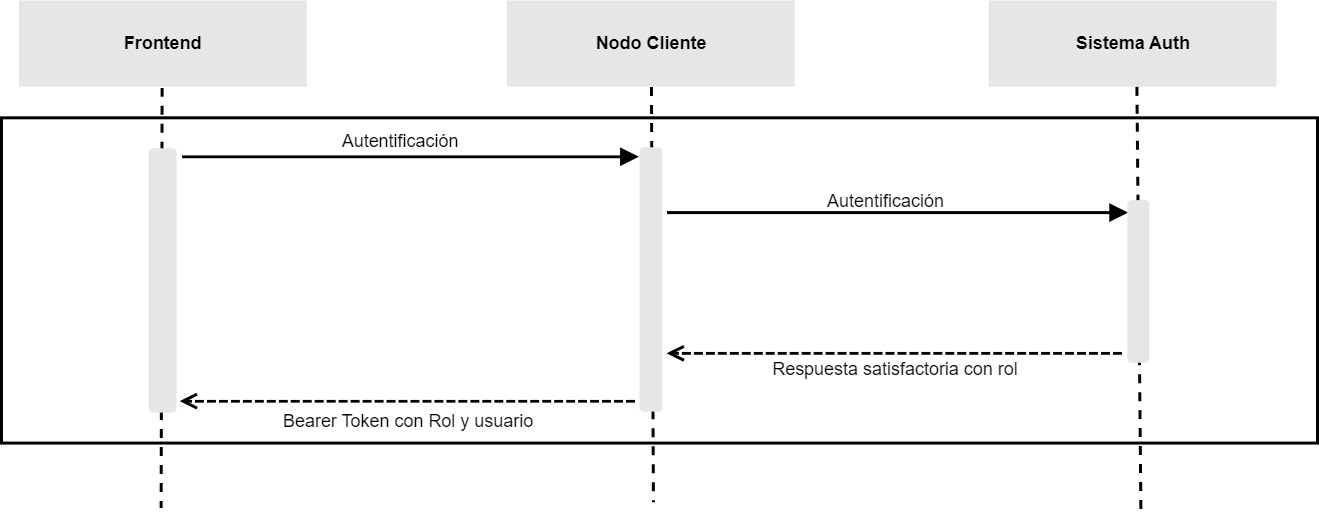
\includegraphics[width=\textwidth]{Graphics/authtt}
\caption{Diagrama de secuencia del proceso de autentificación del sistema.}
\label{fig:autht}
\end{figure}
% ---------------------------------- seguridad
Como se había mencionado previamente en la definición de actores del sistema, los gestores son usuarios registrados en el sistema y además cuentan con un rol definido en dicho sistema. La interfaz de usuario que se propone debe ser capaz de mostrar visualmente las secciones del \textit{back office} relacionadas a los permisos asociados al rol del usuario autenticado.

%JSON Web Token es una forma alternativa de autorizar usuarios a la forma tradicional de usar sesiones. Tradicionalmente, los identificadores de sesión se almacenan en el servidor y se transmiten a la \textit{cookie} del cliente. Cuando el cliente realiza una solicitud al servidor, la identificación de la sesión del cliente se pasa a través del campo de encabezado en la solicitud HTTP al servidor. Luego, el servidor compara la identificación de la sesión recibida del cliente con la almacenada en el servidor. Si coinciden, la solicitud se resuelve; si no, la solicitud se rechaza.

La autentificación de portador (también llamada autenticación de token) es un esquema de autentificación HTTP que involucra tokens de seguridad llamados \textit{Bearer tokens} [\cite{98}]. El nombre ``Autenticación de portador'' puede entenderse como ``dar acceso al portador de este token''. El \textit{Bearer token} es una cadena críptica, generalmente generada por el servidor en respuesta a una solicitud de inicio de sesión.

Tanto el servidor, como el sitio web, se centran en la seguridad. Entre otras cosas: el servidor creará y verificará tokens de identificación (\textit{Bearer token}) para cada usuario, y la interfaz los usará para saber quién está identificado en cada momento y los permisos asociados a ellos; todas las contraseñas de los usuarios se guardarán en formato hash usando la función bcrypt; y, por último, todos los datos recibidos por el servidor se validarán para evitar usos incorrectos.

%JWT opera de una manera diferente. Un token solo se almacena en el lado del cliente de la aplicación, y no en el servidor. En cuanto a la escalabilidad, es mejor usar JWT para autorizar solicitudes, ya que no se almacena en el servidor, por lo tanto, no utiliza la memoria del servidor.

El diagrama \ref{fig:autht} contiene una propuesta de cómo se debe realizar el proceso de autenticación y la interacción de cada parte.

%
%Se envía un token JWT a través de la solicitud HTTP al servidor. Luego, el servidor decodifica y valida el token. Si se valida el token, se resuelve la solicitud, si no, se rechaza la solicitud. JWT es propuesto como un estándar abierto por IETF y es elegido por muchos como la tecnología de referencia para la autorización.
%JWT hace que la autorización sea fácil e intuitiva

\subsection{Diagrama de despliegue}
Un modelo de despliegue consiste en una representación estructural de la arquitectura del sistema desde el punto de vista de la distribución de los artefactos del software en los destinos de despliegue; definiendo a los artefactos como representaciones de elementos concretos en el mundo físico que son el resultado de un proceso de desarrollo [\cite{91}]. 

\begin{figure}[htbp]
\centering
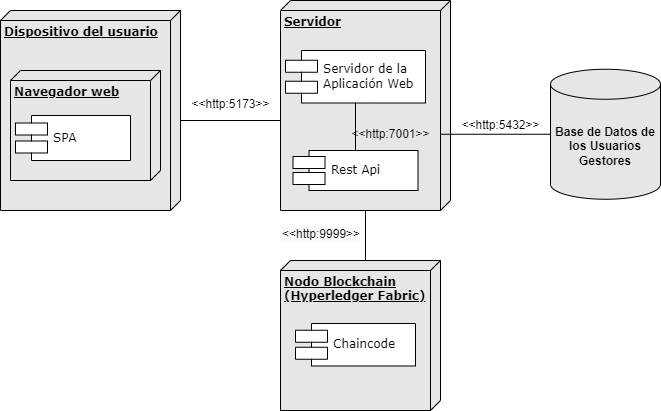
\includegraphics[scale=0.65]{Graphics/deploy}
\caption{Diagrama de despliegue del sistema.}
\label{fig:deploy}
\end{figure}

%Como ya hemos indicado en el apartado anterior, Vue es el framework elegido para la 
%parte del servidor Web. Este framework se apoya en NodeJs, que es un entorno de 
%ejecución de JavaScript orientado a eventos asíncronos, y que será la base para la 
%construcción del módulo Front-End. A su vez, para la creación de los servicios REST 
%desde el componente de la interfaz web, se utiliza Axios, un cliente HTTP basado en 
%promesas para Javascript.
%Estas llamadas serán recibidas por el Back-End, 

%A continuación, se muestra el diagrama de despliegue 
%propuesto para el Portafirmas Digital. El mismo, muestra la disposición física de los nodos que componen 
%el sistema y el reparto de los componentes en dichos nodos.
